% !TEX root = ../main.tex
\chapter{Deep learning for 2D structure prediction}
\label{cap2}

This chapter provides the theoretical foundation necessary to understand the computational approaches utilized in this project. It begins with a brief biological background on proteins and the folding problem, subsequently introducing the simplified lattice model used to represent them computationally. The chapter then explores classical optimization methods explaining each one individually before delving into the core artificial intelligence techniques, namely Reinforcement Learning and Deep Reinforcement Learning, that form the basis of the predictive models developed in this work.

% ─────────────────────────────────────────────────────────────────────
\section{Proteins}
\label{cap2:sec_proteins}

Proteins are large, complex macromolecules that play many critical roles in the body. They do most of the work in cells and are required for the structure, function, and regulation of the body's tissues and organs. A protein is constructed from a set of 20 standard amino acids, linked together in a linear chain known as the \textit{primary structure}.

The functionality of a protein is highly dependent on its specific three-dimensional shape, which it spontaneously adopts through a process called \textbf{protein folding}. Understanding how a sequence of amino acids dictates the final 3D structure the so-called ``Protein Folding Problem'' is a major pursuit in computational biology.

To make the folding problem computationally tractable, researchers often use simplified lattice models. The most prominent of these is the \textbf{Hydrophobic-Polar (HP) model}, introduced by Ken Dill~\cite{dill1985theory}. In the HP model, the 20 amino acids are abstracted into two classes based on their affinity for water:
\begin{itemize}
    \item \textbf{Hydrophobic (H):} water-repelling amino acids (e.g.\ Alanine, Cysteine, Phenylalanine, Isoleucine, Leucine, Methionine, Valine, Tryptophan, Tyrosine).
    \item \textbf{Polar (P):} water-attracting amino acids (all remaining residues).
\end{itemize}
The folding process is driven by the hydrophobic effect, where H monomers tend to cluster together in the core of the structure to minimize exposure to the aqueous environment.

% ─────────────────────────────────────────────────────────────────────
\section{The HP lattice model}
\label{cap2:sec_hp_model}

In a 2D square lattice HP model, a protein sequence of length $n$ is embedded on a 2D integer grid. Each amino acid $i$ occupies a distinct lattice site $(x_i, y_i) \in \mathbb{Z}^2$, and consecutive residues must occupy adjacent lattice sites (i.e.\ $\|p_i - p_{i+1}\|_1 = 1$). The chain must form a \textbf{self-avoiding walk} (SAW): no two residues can share the same lattice site.

\subsection{Neighbour definition}
\label{cap2:subsec_neighbours}

Two residues $i$ and $j$ are defined as \textbf{topological neighbours} if:
\begin{enumerate}
    \item They occupy adjacent grid sites, i.e.\ $|x_i - x_j| + |y_i - y_j| = 1$ (Manhattan distance of 1), \textbf{and}
    \item They are \textbf{non-consecutive} in the primary sequence, i.e.\ $|i - j| > 1$.
\end{enumerate}
This distinction is fundamental: consecutive residues are bonded by the peptide backbone (covalent bond), while non-consecutive residues that happen to be spatially adjacent form \textbf{topological contacts}. Only these non-covalent contacts contribute to the free energy of the conformation.

\subsection{Energy function}
\label{cap2:subsec_energy}

The objective function to be minimized is the \textbf{HP energy}:
\begin{equation}
    E(\mathcal{C}) = -\sum_{\substack{i < j \\ |i-j|>1}} \mathbb{1}[d(p_i, p_j) = 1] \cdot \mathbb{1}[\text{type}(i) = \text{H}] \cdot \mathbb{1}[\text{type}(j) = \text{H}]
    \label{eq:hp_energy}
\end{equation}
where $\mathcal{C}$ denotes a conformation (a set of lattice positions), $d(p_i, p_j)$ is the Manhattan distance between residues $i$ and $j$, and $\mathbb{1}[\cdot]$ is the indicator function. Each H-H topological contact contributes $-1$ to the total energy; a lower (more negative) energy indicates a more stable, compact structure.



Finding the global minimum of $E(\mathcal{C})$ in the HP model is known to be NP-complete~\cite{crescenzi1998complexity}. Consequently, exact algorithms are computationally prohibitive for sequences longer than approximately 15 residues, necessitating the use of heuristic or learned optimization methods.

% ─────────────────────────────────────────────────────────────────────
\section{Move set}
\label{cap2:sec_moveset}

To explore the conformation space, all algorithms in this project use a shared set of \textbf{local moves} that alter the protein structure while preserving chain connectivity and the self-avoiding walk constraint:

\begin{itemize}
    \item \textbf{End-flip:} The first or last residue of the chain is repositioned to one of the free lattice sites adjacent to its sole bonded neighbour. This move only affects a single terminal residue and is applicable at any time.
    \item \textbf{Kink-jump:} Applicable when an internal residue $i$ forms a 90$^\circ$ bend (a ``kink''), i.e.\ when $|x_{i-1} - x_{i+1}| = |y_{i-1} - y_{i+1}| = 1$. The residue is flipped to the diagonally opposite corner of the $2 \times 2$ square formed by $p_{i-1}$, $p_i$, and $p_{i+1}$.
    \item \textbf{Crankshaft:} Applicable when two adjacent internal residues $i$ and $i+1$ form a U-shape, i.e.\ when $\|p_{i-1} - p_{i+2}\|_1 = 1$. Both residues are simultaneously rotated 180$^\circ$ around the axis defined by $p_{i-1}$ and $p_{i+2}$.
    \item \textbf{Pivot:} A pivot point $k$ is selected at random, and all residues from $k+1$ to $n-1$ are rotated by $\pm 90^\circ$ or $180^\circ$ around $p_k$. The move is accepted only if the resulting conformation is self-avoiding (i.e.\ all $n$ positions remain distinct).
\end{itemize}

In the implementation, the four move types are sampled with weights $[0.2, 0.3, 0.3, 0.2]$ to favour the more local (and therefore more frequently valid) kink-jump and crankshaft moves over the more destructive pivot.

\begin{figure}[htbp]
\centering
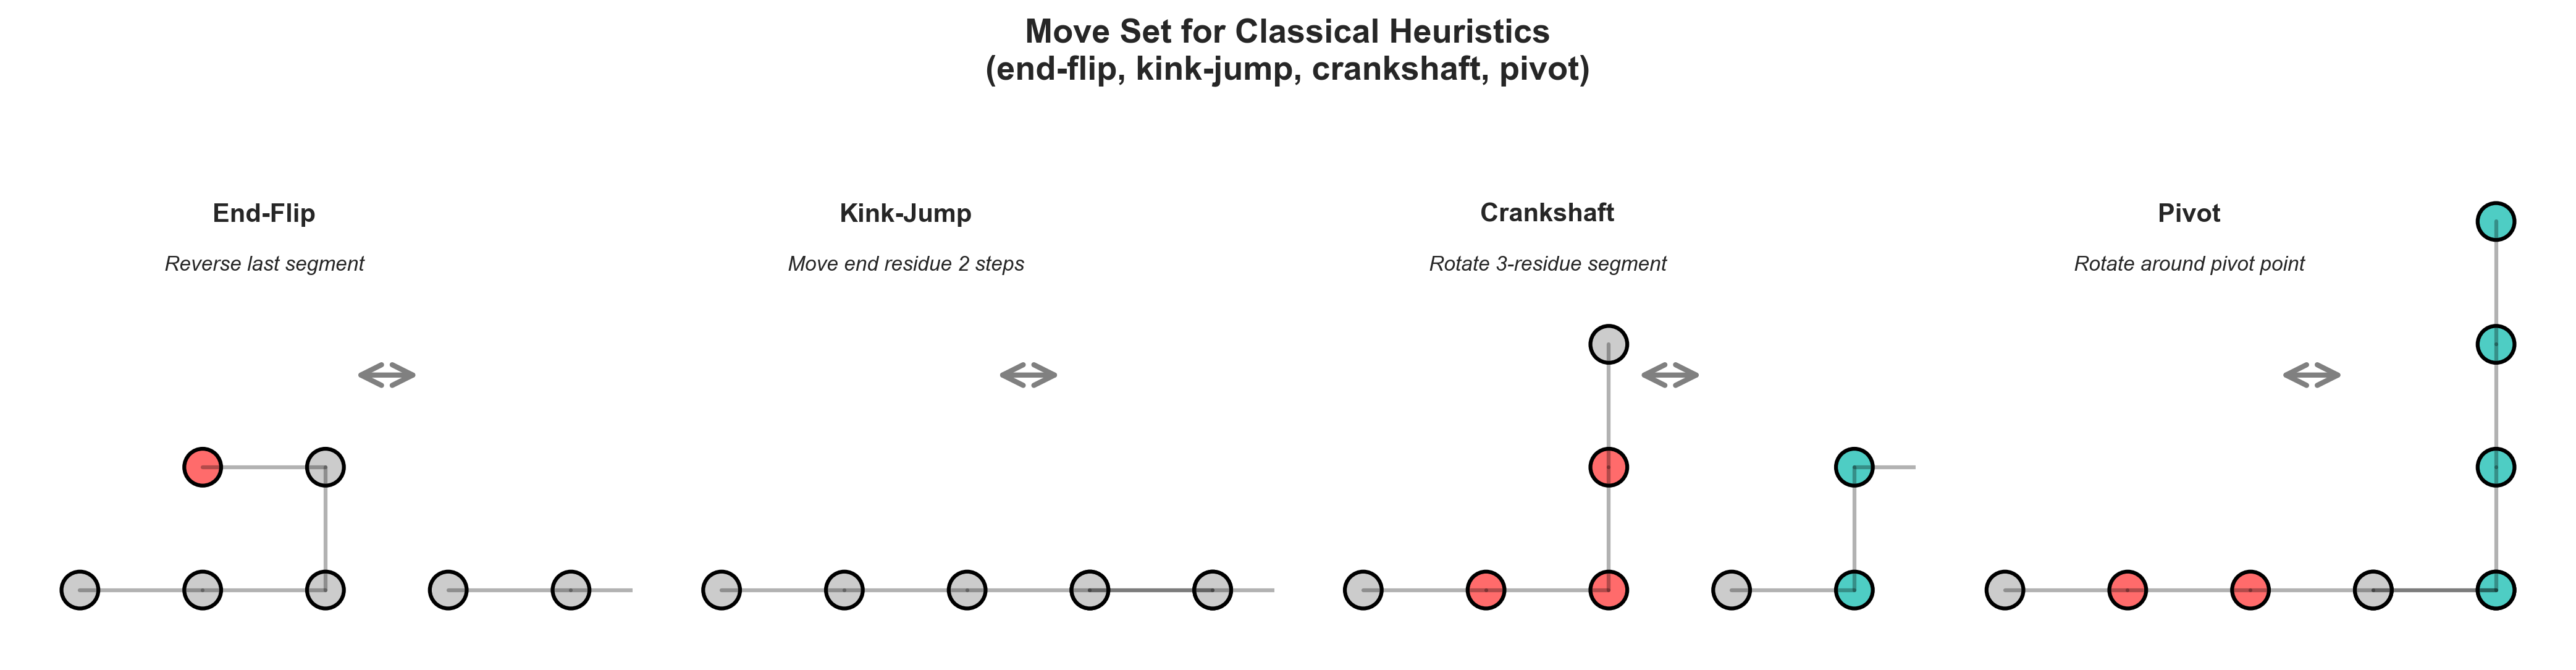
\includegraphics[width=\textwidth]{Figuras/move_set.png}
\caption[Classical heuristic move set]{Move set used by the classical heuristics. The highlighted residues show the part of the chain affected by each local perturbation.}
\label{fig:move_set}
\end{figure}

% ─────────────────────────────────────────────────────────────────────
\section{Classical optimization methods}
\label{cap2:sec_comp_methods}

Because exact enumeration is infeasible, three classical heuristic search algorithms were implemented and benchmarked as baselines.

\subsection{Hill Climbing}
\label{cap2:subsec_hc}

\textbf{Hill Climbing (HC)} is a greedy local search algorithm. Starting from an initial straight-line conformation, it iteratively proposes a random move from the move set and \textbf{accepts it only if the new energy is non-increasing}:
\begin{equation}
    \text{Accept if } E(\mathcal{C}') \leq E(\mathcal{C})
    \label{eq:hc_accept}
\end{equation}
The algorithm maintains a global best solution throughout the search. Although HC is computationally efficient and converges rapidly, it is highly susceptible to \textbf{local minima}: once the algorithm reaches a conformation from which no single move leads to an improvement, the search stalls.

\begin{algorithm}[H]
\caption{Hill Climbing for HP folding}
\label{alg:hc}
\begin{algorithmic}[1]
\State $\mathcal{C} \leftarrow$ straight-line conformation
\State $E_{\text{best}} \leftarrow E(\mathcal{C})$
\For{$t = 1$ \textbf{to} $T_{\max}$}
    \State $m \sim \text{Uniform}(\{\text{end-flip, kink-jump, crankshaft, pivot}\})$
    \State $\mathcal{C}' \leftarrow \text{apply}(m, \mathcal{C})$  \Comment{returns \texttt{None} if invalid}
    \If{$\mathcal{C}' \neq \texttt{None}$ \textbf{and} $E(\mathcal{C}') \leq E(\mathcal{C})$}
        \State $\mathcal{C} \leftarrow \mathcal{C}'$
        \If{$E(\mathcal{C}) < E_{\text{best}}$}
            \State $E_{\text{best}} \leftarrow E(\mathcal{C})$; save best conformation
        \EndIf
    \EndIf
\EndFor
\State \Return best conformation, $E_{\text{best}}$
\end{algorithmic}
\end{algorithm}

\subsection{Simulated Annealing}
\label{cap2:subsec_sa}

\textbf{Simulated Annealing (SA)}, inspired by the metallurgical process of annealing, extends HC by occasionally accepting moves that \textit{worsen} the energy~\cite{kirkpatrick1983optimization}. This probabilistic acceptance criterion allows the search to escape local minima early in the process. The key idea is a temperature parameter $T$ that decreases over time according to a \textbf{cooling schedule}.

A candidate move is accepted with probability:
\begin{equation}
    P(\text{accept}) =
    \begin{cases}
        1 & \text{if } \Delta E \leq 0 \\
        e^{-\Delta E / T} & \text{if } \Delta E > 0
    \end{cases}
    \label{eq:sa_accept}
\end{equation}
where $\Delta E = E(\mathcal{C}') - E(\mathcal{C})$. When the temperature $T$ is high, even largely worse moves are accepted, promoting broad exploration. As $T \rightarrow 0$, the algorithm becomes equivalent to HC.

In this project, an \textbf{exponential cooling schedule} is used:
\begin{equation}
    T_i = T_0 \cdot \left(\frac{T_f}{T_0}\right)^{i / (T_{\max} - 1)}
    \label{eq:sa_cooling}
\end{equation}
where $T_0 = 10.0$ is the initial temperature, $T_f = 0.01$ is the final temperature, and $i$ is the current iteration index.

\begin{algorithm}[H]
\caption{Simulated Annealing for HP folding}
\label{alg:sa}
\begin{algorithmic}[1]
\State $\mathcal{C} \leftarrow$ straight-line conformation; $T \leftarrow T_0$
\For{$t = 1$ \textbf{to} $T_{\max}$}
    \State $T \leftarrow T_0 \cdot (T_f / T_0)^{t/(T_{\max}-1)}$  \Comment{exponential cooling}
    \State $m \sim \text{Uniform}(\text{move set})$; $\mathcal{C}' \leftarrow \text{apply}(m, \mathcal{C})$
    \If{$\mathcal{C}' \neq \texttt{None}$}
        \State $\Delta E \leftarrow E(\mathcal{C}') - E(\mathcal{C})$
        \If{$\Delta E \leq 0$ \textbf{or} $\text{Uniform}(0,1) < e^{-\Delta E / T}$}
            \State $\mathcal{C} \leftarrow \mathcal{C}'$
        \EndIf
        \If{$E(\mathcal{C}) < E_{\text{best}}$}
            \State $E_{\text{best}} \leftarrow E(\mathcal{C})$; save best conformation
        \EndIf
    \EndIf
\EndFor
\State \Return best conformation, $E_{\text{best}}$
\end{algorithmic}
\end{algorithm}

\subsection{Monte Carlo and Replica Exchange Monte Carlo}
\label{cap2:subsec_mc}

\textbf{Monte Carlo (MC)} methods are closely related to SA but operate at a \textit{constant} temperature, using the Metropolis criterion (Equation~\ref{eq:sa_accept}) to accept or reject moves~\cite{metropolis1953equation}. Because the temperature does not change, MC is particularly useful for sampling the thermodynamic ensemble of conformations at a given temperature $T$.

\textbf{Replica Exchange Monte Carlo (REMC)}, also known as parallel tempering, addresses the limitation of single-temperature MC by running $N$ independent MC replicas in parallel, each at a different temperature $T_1 < T_2 < \cdots < T_N$~\cite{hukushima1996exchange,thachuk2007replica}. Periodically, adjacent replicas $k$ and $k+1$ attempt to \textbf{swap} their conformations with probability:
\begin{equation}
    P(\text{swap}) = \min\!\left(1,\; e^{(\beta_k - \beta_{k+1})(E_k - E_{k+1})}\right)
    \label{eq:remc_swap}
\end{equation}
where $\beta_k = 1/T_k$. This exchange mechanism allows low-temperature replicas (which exploit good solutions) to benefit from configurations discovered by high-temperature replicas (which explore broadly), vastly improving the sampling of the energy landscape.

% ─────────────────────────────────────────────────────────────────────
\section{Reinforcement learning}
\label{cap2:sec_rl}

While heuristic algorithms search the energy landscape directly through stochastic perturbations, \textbf{Reinforcement Learning (RL)} approaches the problem differently by training an \textit{agent} to learn \textit{how} to fold a protein through interaction with the environment~\cite{sutton2018reinforcement}.

\subsection{Markov Decision Process formulation}
\label{cap2:subsec_mdp}

The HP folding problem is formulated as a \textbf{Markov Decision Process (MDP)} defined by the tuple $(\mathcal{S}, \mathcal{A}, \mathcal{R}, \mathcal{P}, \gamma)$:

\begin{itemize}
    \item \textbf{State space $\mathcal{S}$:} Each state $s \in \mathcal{S}$ represents the current conformation of the protein chain. In the tabular implementation, this is encoded as a canonical tuple of $(x,y)$ positions, normalized for translation and one rotation symmetry, so that equivalent conformations map to the same state. In the DQN implementation (constructive approach), the state is a rotation-invariant $21 \times 21$ two-channel grid relative to the chain head and current direction.
    \item \textbf{Action space $\mathcal{A}$:} In the classical algorithms (HC, SA, MC, REMC), the agent chooses one of four move types: $\mathcal{A} = \{\text{end-flip},\, \text{kink-jump},\, \text{crankshaft},\, \text{pivot}\}$. In the constructive DQN approach, actions represent relative directions for the next residue: $\mathcal{A} = \{\text{Forward},\, \text{Left},\, \text{Right}\}$, where rotations are applied to the current direction vector.
    \item \textbf{Reward function $\mathcal{R}$:} The reward received after taking action $a$ in state $s$ and transitioning to state $s'$ is:
    \begin{equation}
        R(s, a) =
        \begin{cases}
            E(s) - E(s') & \text{if the move is valid } (= \Delta E > 0 \text{ means energy reduction})\\
            -1 & \text{if the move is invalid (collision / no valid position)}
        \end{cases}
        \label{eq:reward}
    \end{equation}
    This reward is positive when the new conformation has a lower energy (more H-H contacts), zero when energy is unchanged, and negative for invalid moves. The agent therefore learns to prefer energy-reducing moves and to avoid collisions.
    \item \textbf{Discount factor $\gamma \in [0,1)$:} Controls how much the agent values future rewards relative to immediate ones. The tabular implementation used $\gamma = 0.95$, while the DQN training run used $\gamma = 0.99$.
\end{itemize}

\subsection{Tabular Q-Learning}
\label{cap2:subsec_qlearning}

\textbf{Tabular Q-Learning} is a model-free, off-policy RL algorithm~\cite{watkins1992qlearning}. The agent maintains a table (the \textit{Q-table}) $Q: \mathcal{S} \times \mathcal{A} \rightarrow \mathbb{R}$, where $Q(s, a)$ represents the expected cumulative discounted reward obtained by taking action $a$ in state $s$ and then following the optimal policy. Q-values are updated iteratively using the \textbf{Bellman equation}:

\begin{equation}
    Q(s,a) \leftarrow Q(s,a) + \alpha \left[ R(s,a) + \gamma \max_{a'} Q(s',a') - Q(s,a) \right]
    \label{eq:qlearning}
\end{equation}

where $\alpha \in (0,1]$ is the \textit{learning rate} (set to $0.1$) that controls how quickly new information overrides old estimates, and $\gamma = 0.95$ is the discount factor. The term $R(s,a) + \gamma \max_{a'} Q(s',a')$ is called the \textit{TD target} (Temporal Difference target), and $\delta = \text{TD target} - Q(s,a)$ is the \textit{TD error}.

Action selection follows an \textbf{$\varepsilon$-greedy policy}: with probability $\varepsilon$ the agent selects a random action (exploration), and with probability $1 - \varepsilon$ it selects the action with the highest Q-value (exploitation). The exploration rate $\varepsilon$ is decayed linearly from $1.0$ to $0.05$ over the first half of training:

\begin{equation}
    \varepsilon_t = \max\!\left(\varepsilon_{\min},\; \varepsilon_0 - (\varepsilon_0 - \varepsilon_{\min}) \cdot \frac{t}{\lfloor T_{\text{decay}} \rfloor}\right)
    \label{eq:epsilon_decay}
\end{equation}

where $T_{\text{decay}} = \lfloor \text{episodes} \times \text{steps\_per\_episode} / 2 \rfloor$.

\begin{algorithm}[H]
\caption{Tabular Q-Learning for HP folding}
\label{alg:ql}
\begin{algorithmic}[1]
\State Initialize $Q(s,a) \leftarrow 0$ for all $s, a$; $\varepsilon \leftarrow 1.0$
\For{each episode}
    \State $\mathcal{C} \leftarrow$ straight-line conformation; $s \leftarrow \text{encode}(\mathcal{C})$
    \For{each step}
        \State Decay $\varepsilon$ according to Equation~\ref{eq:epsilon_decay}
        \If{$\text{Uniform}(0,1) < \varepsilon$}
            \State $a \leftarrow \text{random action}$ \Comment{explore}
        \Else
            \State $a \leftarrow \arg\max_{a'} Q(s, a')$ \Comment{exploit}
        \EndIf
        \State $\mathcal{C}' \leftarrow \text{apply}(a, \mathcal{C})$
        \State Compute reward $R$ via Equation~\ref{eq:reward}
        \State $s' \leftarrow \text{encode}(\mathcal{C}')$
        \State $Q(s,a) \leftarrow Q(s,a) + \alpha[R + \gamma \max_{a''} Q(s',a'') - Q(s,a)]$
        \State $s \leftarrow s'$; $\mathcal{C} \leftarrow \mathcal{C}'$; update global best
    \EndFor
\EndFor
\State \Return best conformation, $E_{\text{best}}$, $Q$-table
\end{algorithmic}
\end{algorithm}

Tabular Q-Learning is effective for short sequences (up to $\approx 25$ residues) but suffers from the \textit{curse of dimensionality}: the number of distinct conformations grows exponentially with chain length, making the Q-table intractably large for realistic proteins.

% ─────────────────────────────────────────────────────────────────────
\section{Deep reinforcement learning}
\label{cap2:sec_drl}

\textbf{Deep Reinforcement Learning (DRL)} overcomes the scalability limitation by replacing the Q-table with a parametric function approximator: a \textbf{Deep Q-Network (DQN)} introduced by Mnih et al.~\cite{mnih2015human}. Instead of storing one Q-value per state-action pair, the network $Q(s, a; \theta)$ with parameters $\theta$ maps a state representation directly to a vector of Q-values for all actions.

\subsection{State representation}
\label{cap2:subsec_state_rep}

In the constructive DQN implementation, the state is encoded as a two-channel grid of size $21 \times 21$ (nine times smaller, focusing only on the local neighborhood). The encoding is rotation-invariant: the grid is centered on the chain's head (last positioned residue) and rotated so that the current direction vector always points upward. Each channel encodes residue type:
\begin{equation}
    g_{\text{channel}}[x, y] =
    \begin{cases}
        1.0 & \text{if a residue of the corresponding type occupies the rotated position } (x, y) \\
        0.0  & \text{(empty site)}
    \end{cases}
    \label{eq:grid_encoding_new}
\end{equation}
Channel 0 represents Hydrophobic (H) residues, channel 1 represents Polar (P) residues. This rotation-invariant encoding dramatically reduces state space size while ensuring that the CNN learns folding patterns that are independent of the chain's global position and orientation, enabling better generalization across proteins of different lengths and H-content.

\subsection{Network architecture}
\label{cap2:subsec_cnn}

The neural network is a \textbf{Convolutional Neural Network (CNN)} designed to process $2 \times 21 \times 21$ inputs. The final architecture used in the Colab-trained model consists of:

\begin{enumerate}
    \item \textbf{Input:} Two-channel grid ($2 \times 21 \times 21$) representing H and P residue positions.
    \item \textbf{Convolutional block 1:} \texttt{Conv2d}($2, 32$, kernel $3\times3$, padding $1$) $\rightarrow$ \texttt{ReLU}. Output: $32 \times 21 \times 21$.
    \item \textbf{Convolutional block 2:} \texttt{Conv2d}($32, 64$, kernel $3\times3$, padding $1$) $\rightarrow$ \texttt{ReLU}. Output: $64 \times 21 \times 21$.
    \item \textbf{Convolutional block 3:} \texttt{Conv2d}($64, 64$, kernel $3\times3$, padding $1$) $\rightarrow$ \texttt{ReLU}. Output: $64 \times 21 \times 21$.
    \item \textbf{Flatten:} $64 \times 21 \times 21 = 28{,}224$ features.
    \item \textbf{Fully connected:} \texttt{Linear}($28224, 256$) $\rightarrow$ \texttt{ReLU} $\rightarrow$ \texttt{Linear}($256, 3$).
\end{enumerate}

The output layer produces 3 Q-values, one per relative direction action (Forward, Left, Right). The compact $21 \times 21$ grid dramatically reduces memory overhead while focusing on local patterns. Combined with the rotation-invariant encoding, this architecture enables the CNN to learn generalizable folding strategies that transfer effectively across proteins of different lengths and compositions.

\begin{figure}[htbp]
\centering
\small
\setlength{\tabcolsep}{3pt}
\resizebox{\textwidth}{!}{%
\begin{tabular}{ccccccccccccc}
\fcolorbox{black}{blue!10}{\parbox[c][2.3cm][c]{2.5cm}{\centering
\textbf{Input State}\\
$2 \times 21 \times 21$\\
H/P channels\\
\footnotesize rotation-invariant grid}}
& $\rightarrow$ &
\fcolorbox{black}{green!12}{\parbox[c][2.3cm][c]{2.5cm}{\centering
\textbf{Conv2D + ReLU}\\
$2 \rightarrow 32$\\
$3 \times 3$, padding 1\\
\footnotesize $32 \times 21 \times 21$}}
& $\rightarrow$ &
\fcolorbox{black}{green!12}{\parbox[c][2.3cm][c]{2.5cm}{\centering
\textbf{Conv2D + ReLU}\\
$32 \rightarrow 64$\\
$3 \times 3$, padding 1\\
\footnotesize $64 \times 21 \times 21$}}
& $\rightarrow$ &
\fcolorbox{black}{green!12}{\parbox[c][2.3cm][c]{2.5cm}{\centering
\textbf{Conv2D + ReLU}\\
$64 \rightarrow 64$\\
$3 \times 3$, padding 1\\
\footnotesize $64 \times 21 \times 21$}}
& $\rightarrow$ &
\fcolorbox{black}{yellow!20}{\parbox[c][2.3cm][c]{2.0cm}{\centering
\textbf{Flatten}\\
28,224\\
features}}
& $\rightarrow$ &
\fcolorbox{black}{orange!15}{\parbox[c][2.3cm][c]{2.0cm}{\centering
\textbf{FC + ReLU}\\
$28{,}224 \rightarrow 256$}}
& $\rightarrow$ &
\fcolorbox{black}{red!12}{\parbox[c][2.3cm][c]{1.8cm}{\centering
\textbf{Output}\\
$256 \rightarrow 3$\\
Q-values\\
\footnotesize F/L/R}}
\end{tabular}%
}

\vspace{0.6em}

\resizebox{0.9\textwidth}{!}{%
\begin{tabular}{cccc}
\fcolorbox{black}{gray!12}{\parbox[c][1.15cm][c]{3.0cm}{\centering
\textbf{Replay Buffer}\\
100,000 transitions}}
&
\fcolorbox{black}{gray!12}{\parbox[c][1.15cm][c]{3.2cm}{\centering
\textbf{Target Network}\\
sync every 1,000 optimization steps}}
&
\fcolorbox{black}{gray!12}{\parbox[c][1.15cm][c]{3.0cm}{\centering
\textbf{Exploration}\\
$\varepsilon$: $1.0 \rightarrow 0.05$}}
&
\fcolorbox{black}{gray!12}{\parbox[c][1.15cm][c]{3.0cm}{\centering
\textbf{Stabilization}\\
Double DQN + clipping 10}}
\end{tabular}%
}
\caption[Constructive DQN architecture]{Constructive DQN architecture used for residue-by-residue folding. The two input channels encode hydrophobic and polar residues, and the output layer estimates Q-values for the relative actions Forward, Left and Right.}
\label{fig:dqn_architecture}
\end{figure}

\subsection{Training procedure}
\label{cap2:subsec_dqn_training}

DQN training relies on key stabilization mechanisms:

\begin{itemize}
    \item \textbf{Constructive Environment:} Unlike perturbative approaches that start with a straight line and modify it, the constructive environment builds the protein one amino acid at a time. The first two residues are positioned to define an initial direction; subsequent residues are placed via relative direction decisions (Forward/ Left/ Right). This guarantees self-avoiding walks by design and simplifies the state space.
    \item \textbf{Experience Replay:} Transitions $(s, a, r, s')$ are stored in a \textit{Replay Buffer} of capacity $100{,}000$. At each training step, a random mini-batch (batch size 128) is sampled. This breaks temporal correlations and reduces gradient variance.
    \item \textbf{Target Network:} A separate network copy, $Q(s, a; \theta^-)$, computes TD targets. Its weights $\theta^-$ are synchronized every 1,000 optimization steps, preventing oscillations from constantly moving targets.
    \item \textbf{Reward Structure:} $R = +1.0$ for each new H-H contact formed (direct energy feedback), $-1.0$ for invalid moves (collisions), $+0.5$ bonus for completing the full chain without collision, with additional shaping for low-H-density proteins.
    \item \textbf{Stability Mechanisms:} The training loop uses Double DQN target selection and gradient clipping with maximum norm 10.
\end{itemize}

The loss function is the \textbf{Mean Squared Error (MSE)} between predicted and target Q-values. In the final implementation, the target action is selected by the policy network and evaluated by the target network, following the Double DQN formulation:
\begin{equation}
    a^* = \arg\max_{a'} Q(s', a'; \theta)
    \quad ; \quad
    y = r + \gamma Q(s', a^*; \theta^-)(1-done)
    \quad ; \quad
    \mathcal{L}(\theta) = \mathbb{E}_{(s,a,r,s') \sim \mathcal{D}} \left[ \left( y - Q(s, a; \theta) \right)^2 \right]
    \label{eq:dqn_loss}
\end{equation}
Network parameters $\theta$ are optimized via \textbf{Adam}~\cite{kingma2015adam} with learning rate $\eta = 0.001$, $\gamma = 0.99$, and $\varepsilon$-decay from 1.0 to 0.05 over training. Training is performed on a dataset of 20 real UniProt proteins for 20,000 episodes, with GPU acceleration available.

\begin{algorithm}[H]
\caption{Constructive Deep Q-Network for HP folding}
\label{alg:dqn_constructive}
\begin{algorithmic}[1]
\State Initialize policy network $Q(s,a;\theta)$ and target network $Q(s,a;\theta^-)$
\State Copy initial weights: $\theta^- \leftarrow \theta$
\State Initialize replay buffer $\mathcal{D}$ with capacity $100{,}000$
\State Set $\varepsilon \leftarrow 1.0$, $\varepsilon_{\min} \leftarrow 0.05$, $\gamma \leftarrow 0.99$
\For{episode $= 1$ to $20{,}000$}
    \State Sample one HP sequence from the training set
    \State Reset constructive environment with first two residues fixed
    \While{the chain is not complete and no collision occurred}
        \State Encode partial chain as a $2 \times 21 \times 21$ rotation-invariant grid $s$
        \If{$\mathrm{Uniform}(0,1) < \varepsilon$}
            \State Select random action $a \in \{\text{Forward}, \text{Left}, \text{Right}\}$
        \Else
            \State Select $a = \arg\max_{a'} Q(s,a';\theta)$
        \EndIf
        \State Apply $a$ to place the next residue and observe $(r, s', done)$
        \State Store transition $(s,a,r,s',done)$ in $\mathcal{D}$
        \If{$|\mathcal{D}|$ is larger than the mini-batch size}
            \State Sample a random mini-batch from $\mathcal{D}$
            \State Select $a^* = \arg\max_{a'} Q(s',a';\theta)$ and compute $y = r + \gamma Q(s',a^*;\theta^-)(1-done)$
            \State Update $\theta$ by minimizing $\left(y - Q(s,a;\theta)\right)^2$
        \EndIf
    \EndWhile
    \State Decay $\varepsilon \leftarrow \max(\varepsilon_{\min}, 0.995\varepsilon)$
    \If{1,000 optimization steps have elapsed}
        \State Synchronize target network: $\theta^- \leftarrow \theta$
    \EndIf
\EndFor
\State Save trained weights to \texttt{dqn\_weights.pth}
\end{algorithmic}
\end{algorithm}

% ─────────────────────────────────────────────────────────────────────
\section{Summary}
\label{cap2:sec_summary}

This chapter detailed the theoretical concepts underlying the computational approaches to the 2D protein folding problem. We began by formalizing the HP lattice model, defining the notion of topological neighbours and the HP energy function. We then described the shared move set (end-flip, kink-jump, crankshaft, pivot) used by all algorithms. For the classical baseline methods, each algorithm was presented individually: Hill Climbing as a fast but locally trapped greedy search, Simulated Annealing as a temperature-controlled stochastic method capable of escaping local minima, and Replica Exchange Monte Carlo as a parallel, multi-temperature approach for robust landscape exploration. Finally, we introduced the Reinforcement Learning paradigm, formally defining the MDP formulation including the state space, action space, and reward function. We traced the evolution from Tabular Q-Learning which learns discrete folding policies via the Bellman equation and $\varepsilon$-greedy exploration to Deep Q-Networks, which replace the Q-table with a CNN capable of processing large spatial grids, offering a scalable method for predicting the structures of complex proteins.
